% formato FRONTE RETRO
\documentclass[epsfig,a4paper,11pt,titlepage,twoside,openany]{book}
\usepackage{epsfig}
\usepackage{plain}
\usepackage{setspace}
\usepackage[paperheight=29.7cm,paperwidth=21cm,outer=1.5cm,inner=2.5cm,top=2cm,bottom=2cm]{geometry} % per definizione layout
\usepackage{titlesec} % per formato custom dei titoli dei capitoli

% custom packages import
\usepackage[acronym]{glossaries}

\makenoidxglossaries
\newacronym{ugvs}{UGVs}{Unmanned Ground Vehicles}
\newacronym{ros}{ROS}{Robot Operating System}
\newacronym{uavs}{UAVs}{Unmanned Aerial Vehicles}
\newacronym{nav2}{Nav2}{ROS2 Navigation Stack}
\newacronym{urdf}{URDF}{Unified Robotic Description Format}
\newacronym{sdf}{SDF}{Simulation Description Format}
\newacronym{rviz}{RViz2}{ROS Visualization Tool 2}
\newacronym{amcl}{AMCL}{Adaptive Monte-Carlo Localization}
\newacronym{slam}{SLAM}{Simultaneous Localization and Mapping}
\newacronym{btnav}{BT Navigator}{Behavior Tree Navigator}
\newacronym{ekf}{EKF}{Extended Kalman Filter}
\newacronym{gui}{GUI}{Graphical User Interface}
\newacronym{disi}{DISI}{Dipartimento di Ingegneria e Scienze dell'Informazione}

\makeatletter
{\catcode`\/=\active
  \gdef\slashbreak{
    \catcode`\/=\active
    \def/{\char`\/\penalty\z@}}
}
\makeatother

\makeatletter
\newcommand\footnoteref[1]{\protected@xdef\@thefnmark{\ref{#1}}\@footnotemark}
\makeatother

\usepackage[dvipsnames]{xcolor}
\usepackage{listings}

\usepackage{filecontents}
\usepackage{graphicx, caption}
\usepackage{wrapfig}
\usepackage{subcaption}

\usepackage{hyperref}

\usepackage{chemarrow}

\usepackage[export]{adjustbox}

\usepackage{tikz}
\tikzset{
  block/.style={rectangle, draw, text width=0.15\textwidth, text centered, rounded corners, minimum height=3em, node distance=0.1\textwidth and 0.25\textwidth},
  inception/.style={rectangle, draw, text width=0.2\textwidth, text centered, rounded corners, minimum height=3em, node distance=0.1\textwidth and 0.25\textwidth},
  arrow/.style={-{Stealth[]}},
  poseserver/.style={rectangle, draw, text width=\textwidth, text centered, rounded corners, minimum height=3em, node distance=0.1\textwidth},
  navigationclient/.style={rectangle, draw, text width=, text centered, rounded corners, minimum height=3em, node distance=0.1\textwidth},
  }
\usetikzlibrary{positioning,arrows.meta,fit}
\usepackage{multicol}

\newcommand{\arguments}[2]{\textbf{#1}: \textit{#2}}

\newif\ifapplymulticol
\makeatletter
\lst@AddToHook{InitVars}{\ifapplymulticol\edef\lst@next{\noexpand\multicols{2}}\expandafter\lst@next\fi}
\lst@AddToHook{ExitVars}{\ifapplymulticol\def\lst@next{\global\let\@checkend\@gobble
                      \endmulticols
                      \global\let\@checkend\lst@@checkend}
        \expandafter\lst@next\fi}
\makeatother

\def\code#1{\texttt{#1}}

\setlength\intextsep{0pt}

\lstdefinelanguage{json}{
    morekeywords=[1]{label, center, max, min},
    morekeywords=[2]{povo_1_258},
    literate=
     *{:}{{{\color{Red}{:}}}}{1}
      {,}{{{\color{Red}{,}}}}{1}
      {\{}{{{\color{Blue}{\{}}}}{1}
      {\}}{{{\color{Blue}{\}}}}}{1}
      {[}{{{\color{Blue}{[}}}}{1}
      {]}{{{\color{Blue}{]}}}}{1}
}

\lstdefinestyle{jsonStile}{
    frame=tb,
    language=json,
    columns=flexible,
    keepspaces=true,
    breaklines=true,
    basicstyle=\small\ttfamily,
    keywordstyle=[1]\color{Green},
    keywordstyle=[2]\color{NavyBlue},
}

\definecolor{ipython_red}{RGB}{186, 33, 33}
\definecolor{ipython_green}{RGB}{0, 128, 0}
\definecolor{ipython_cyan}{RGB}{64, 128, 128}
\definecolor{ipython_purple}{RGB}{170, 34, 255}

\lstdefinestyle{PythonStile}{
    frame=tb,
    language=Python,
    columns=flexible,
    keepspaces=true,
    breaklines=true,
    identifierstyle=\color{black},
    commentstyle=\color{ipython_cyan},
    stringstyle=\color{ipython_red},
    basicstyle=\small\ttfamily,
    keywordstyle=[1]\color{ipython_green},
    keywordstyle=[2]\color{ipython_purple}
}

\lstdefinelanguage{Python}{
    morekeywords=[1]{open, load, dump, dirname, abspath, \_\_file\_\_, import, array, cos, sin, dot, dict},
    sensitive=true,
    morekeywords=[2]{translation, rot\_z, scale\_y, current\_folder, original\_name, dict\_name, original\_data, rot\_matrix, scale\_matrix, roto\_scaling, dict\_data, obj, k, v},
    morecomment=[l]\#,
    morestring=[b]",
}

\lstdefinelanguage{Dockerfile}
{
  morekeywords={FROM, RUN, CMD, LABEL, MAINTAINER, EXPOSE, ENV, ADD, COPY,
    ENTRYPOINT, VOLUME, USER, WORKDIR, ARG, ONBUILD, STOPSIGNAL, HEALTHCHECK,
    SHELL},
  morecomment=[l]{\#},
  morestring=[b]',
  morestring=[b]",
}

\lstdefinestyle{DockerStyle}{
    frame=tb,
    language=Dockerfile,
    columns=flexible,
    keepspaces=true,
    showstringspaces=false,
    basicstyle=\small\ttfamily,
    commentstyle=\color{Gray},
    keywordstyle=\color{Red},
    stringstyle=\color{RoyalBlue},
}

\lstdefinestyle{CStyleTextWidth}{
    language=C,
    columns=flexible,
    keepspaces=true,
    breaklines=true,
    linewidth=\textwidth,
    showstringspaces=false,
    morekeywords=[2]{canTransform, lookupTransform},
    basicstyle=\small\ttfamily,
    commentstyle=\color{Gray},
    keywordstyle=\color{Red},
    keywordstyle=[2]\color{Purple},
    stringstyle=\color{RoyalBlue},
}

\lstdefinestyle{CStyleNoFrame}{
    language=C,
    columns=flexible,
    keepspaces=true,
    breaklines=true,
    showstringspaces=false,
    morekeywords=[2]{send_goal},
    basicstyle=\small\ttfamily,
    commentstyle=\color{Gray},
    keywordstyle=\color{Red},
    keywordstyle=[2]\color{Purple},
    stringstyle=\color{RoyalBlue},
}

\lstdefinestyle{CStyle}{
    language=C,
    frame=tb,
    columns=flexible,
    keepspaces=true,
    breaklines=true,
    showstringspaces=false,
    morekeywords=[2]{this, GOAL_INDEX, room_goal_, goal_position_, future, result, get_pose, continue_work, progress_},
    basicstyle=\small\ttfamily,
    commentstyle=\color{Gray},
    keywordstyle=\color{Red},
    keywordstyle=[2]\color{Purple},
    stringstyle=\color{RoyalBlue},
}

\lstdefinelanguage{xml}{
  morestring=[b]",
  morecomment=[s]{<?}{?>},
  morekeywords={type,pkg,name,args}
}

\lstdefinestyle{xmlStyle}{
    frame=tb,
    language=XML,
    basicstyle=\ttfamily,
    columns=flexible,
    showstringspaces=false,
    commentstyle=\color{gray}\upshape,
    stringstyle=\color{ForestGreen},
    identifierstyle=\color{Red},
    keywordstyle=\color{Black}
}

\lstdefinelanguage{bash}{
    morestring=[b]",
    morecomment=[l]{\#}
}

\lstdefinestyle{bashStyle}{
    frame=tb,
    language=bash,
    basicstyle=\ttfamily,
    columns=flexible,
    showstringspaces=false,
    commentstyle=\color{gray}\upshape,
    stringstyle=\color{Blue},
    keywordstyle=\color{Black}
}

%%%%%%%%%%%%%%
% supporto lettere accentate
%
%\usepackage[latin1]{inputenc} % per Windows;
\usepackage[utf8x]{inputenc} % per Linux (richiede il pacchetto unicode);
%\usepackage[applemac]{inputenc} % per Mac.

\singlespacing

\usepackage[english]{babel}

\begin{document}
% \begin{slashbreak}

  % nessuna numerazione
  \pagenumbering{gobble} 
  \pagestyle{plain}

\thispagestyle{empty}

\begin{center}
  \begin{figure}[h!]
    \centerline{
\psfig{file=marchio_unitrento_colore_it_202002.eps,width=0.6\textwidth}}
  \end{figure}

  \vspace{2 cm} 

  \LARGE{Department of Information Engineering and Computer Science\\}

  \vspace{1 cm} 
  \Large{Bachelor's Degree in\\
    Computer Science
  }

  \vspace{2 cm} 
  \Large\textsc{Final dissertation\\} 
  \vspace{1 cm} 
  \Huge\textsc{Drone Surveillance: a ROS2 solution for ground robots autonomous navigation\\}
  \Large{\it{Both for real and simulated environments (?)}}


  \vspace{2 cm} 
  \begin{tabular*}{\textwidth}{ c @{\extracolsep{\fill}} c }
  \Large{Supervisor} & \Large{Student}\\
  \Large{Palopoli Luigi}& \Large{Franzin Mattia}\\
  \end{tabular*}

  \vspace{2 cm} 

  \Large{Academic year 2021/2022}
  
\end{center}



  \cleardoublepage
 
  \thispagestyle{empty}

\begin{center}
  {\bf \Huge Acknowledgements}
\end{center}

\vspace{4cm}


\emph{
  ...thanks to...
}

  \clearpage
  \pagestyle{plain} % nessuna intestazione e pie pagina con numero al centro
  
  % inizio numerazione pagine in numeri arabi
  \mainmatter
    % indice
    \tableofcontents
    \clearpage
    
    
          
    % gruppo per definizone di successione capitoli senza interruzione di pagina
    \begingroup
      % nessuna interruzione di pagina tra capitoli
      % ridefinizione dei comandi di clear page
      % \renewcommand{\cleardoublepage}{} 
      % \renewcommand{\clearpage}{} 
      % redefinizione del formato del titolo del capitolo
      % da formato
      %   Capitolo X
      %   Titolo capitolo
      % a formato
      %   X   Titolo capitolo
      
      \titleformat{\chapter}
        {\normalfont\Huge\bfseries}{\thechapter}{1em}{}
        
      \titlespacing*{\chapter}{0pt}{0.59in}{0.02in}
      \titlespacing*{\section}{0pt}{0.20in}{0.02in}
      \titlespacing*{\subsection}{0pt}{0.10in}{0.02in} 
      
      \addcontentsline{toc}{chapter}{Abstract} % check inglese (?)

\chapter*{Abstract}
\label{abstract}

Robots nowadays are being employed more and more to help humans in their tasks:  from automating a productive chain to helping people in need, from working in dangerous situation to replacing them in repetitive tasks, saving their time and energy. This thesis discusses the design of a surveillance system making use of ground robots, developed in the past few months during my internship at the Robotic Lab in the University of Trento. 

Using the provided robots, a fully functional system has been developed, and it can be used in the university environments, but not only this. Normally if you want to test new algorithms and technics, you should use the real robots, which means physically being in the Lab, and it is not always possible. Indeed, this project comes also as a playground: it can also run in a simulation, and thanks to the fact the simulated environment has been kept as close as possible to the real one, it does not matter where you are testing things out, they should work without any big difference.

In addition to the navigation system, a planning one developed by another student has been integrated, since the entire project is shared: thanks to a web interface it is possible to specify areas the robots should patrol, the available ones will be assigned to the task and they will move autonomously giving their feedback back at the end.
      \chapter{Introduction} % senza numerazione
\label{cha:intro}

% \addcontentsline{toc}{chapter}{Introduction} % da aggiungere comunque all'indice

\section{Summary}

The purpose of this project is to develop (developing?) a fullstack (?) system for surveillance proposes using mobile robots, both ground and flying ones.
Since the project is quite big (?), it is shared with other two students with each one of us focusing into a specific subtask (?). It is constituted of: 

\begin{itemize}
  \item a planning system, responsible for dispatching the surveillance tasks to UGVs and/or UAVs in the best possible way based on their battery charge, giving them some waypoints to follow in order to follow the optimal path.
  \item a solution to autonomously control the drones (UAVs robots)
  \item a solution to autonomously control ground robots avoiding dynamic obstacles (UGVs robots)
\end{itemize}

Basically, all the work is done using \Acrshort{ros2}\footnote{The Robot Operating System (ROS) is a set of software libraries and tools for building robot applications\cite{ros2desc}} which gives us the possibility to work separately on your own project, and since everyone creates his custom packages, at the end we only need to put everything together.

A more detailed description can be found in the first chapter.

The reason behind my choice about the internship and this consequent thesis is leaded by my growing interest in this topic: just some month before taking part in this work I attended a course about {\it robotic fundamentals}\cite{intro2robotics} in which I had to work in a custom project similar to this, but using a manipulator.

For me, is the possibility to give to some inanimate object, like a wheeled robot or a manipulator, something that could be described as intelligence, the ability to perform some tasks in response of other ones, figuring out which ones are the best for every particular situation. Another aspect I really like is the (inbuilt) utility which carries (within) itself: this is only an educational project, but it is easy to imagine an industrial application, for example for patrol purposes. // ?

Some challenges I decided to took are the choice of the new version of ROS, with some great improves respect to the older one, but with less community support, and also working for the first time with a mobile robot.

% Il sommario dell’elaborato consiste al massimo di 3 pagine e deve contenere le seguenti informazioni:
% \begin{itemize}
%   \item contesto e motivazioni 
%   \item breve riassunto del problema affrontato
%   \item tecniche utilizzate e/o sviluppate
%   \item risultati raggiunti, sottolineando il contributo personale del laureando/a
% \end{itemize}

% Tipo:
% - descrizione tesi e interesse robotica
% - far muovere robot in un ambiente seguendo le istruzioni ricevute ed evitando ostacoli non previsti
% - ROS2, nav2, waypoint follower
% - il robot si muove e fa foto

\section{Other projects involved}

What follows is a brief description of the work done by the other two students to have a better and clear idea of the workflow of the entire system.

\subsection{Planning system}

To be done...

\subsection{Drones control}

To be done...


      \setlength\intextsep{0pt}

\chapter{About the technology stack}
\label{cha:techstack}

Before describing the entire project, we need to know what we are talking about. In particular, there are the software and libraries strongly used in the project:  
\begin{itemize}
    \item ROS2
    \item Gazebo
    \item \acrfull{rviz}
    \item \acrfull{nav2}
    \item Docker
\end{itemize}

\section{\acrshort{ros}2}

\begin{wrapfigure}{l}{0.2\textwidth}
    
\includegraphics[width=0.2\textwidth]{images/foxy}
\end{wrapfigure}

\textit{\acrshort{ros}2, which stands for Robot Operative System 2, is a set of software libraries and tools for building robot applications.}\cite{ros2desc} On it, every process is a node and each node has the possibility to talk to other ones thanks to some channel of communications called topics using the publish/subscribe model.

This version of \acrshort{ros}2, called \textbf{Foxy}, was used because it is possible to integrate the \textit{plansys2} libraries used for planning.

Thanks to \Acrshort{ros} \textit{hardware abstraction, low-level device control, implementation of commonly-used functionality, message-passing between processes, and package management}\cite{ros2help}, the developer can ignore specific hardware details and software implementations and focus only on the application itself. 

This means that executing a \acrshort{ros} node on your own computer is the same of executing it on a robot, as long as you are using the same operative system (only \textbf{Ubuntu 20.04}) and the same external devices, if you are not simulating them.

\section{Gazebo}
\label{sec:gazebo} % add more info about gazebo (?)

\begin{wrapfigure}{r}{0.25\textwidth}
    
\includegraphics[width=0.25\textwidth]{images/gazebo}
\end{wrapfigure}

Gazebo is a simulation suite. It lets you create and simulate things with the bundled physic and render engines, alongside a variety of sensors.

It comes as a standalone software, but thanks to its interfaces it is possible to integrate it with \acrshort{ros}2, using several packages developed for this purpose: in this way you can simulate both robots and the environments in which they operate, before actually moving to the real world, or test your last modifications even if you are somewhere other than the real robot location.

With the sensors and the plugins you are able to simulate lasers (e.g. lidars), cameras (e.g. depth cameras), IMUs and GPS receivers, or also differential drive and joints state.

\section{\acrfull{rviz}}

\begin{wrapfigure}{l}{0.25\textwidth}
    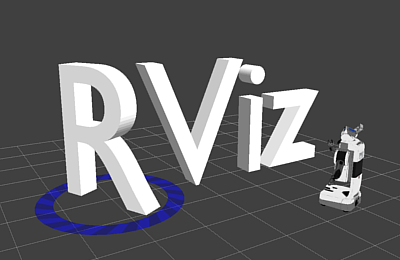
\includegraphics[width=0.25\textwidth]{images/rviz}
\end{wrapfigure}

\Acrshort{rviz}, is a visualization tool for ROS: you can visualize the sensors, the robots, the environment, and also the algorithms; in general, you can see the actual state of your \acrshort{ros} system. In this project it has been used to set initial robot position on the map, see room boundaries, obstacles and visualize the path the robot is currently following to reach the goal, that could be specified graphically (manually) or by some other nodes (automatically). 

\section{\acrfull{nav2}}

The Navigation Stack is a collection of packages of \acrshort{ros}2 providing useful tools for the navigation of your robot: path planning, localization, obstacle avoidance, recovery from collisions, mapping and so on\footnote{A detailed description can be found in \autoref{cha:navigation}.}. These packages were used as a basis for this project: in such a manner you do not have to worry about the navigation algorithms, you just need to pass sensor information, and they will do the rest; moreover, you can use the provided interfaces to customize and automate the whole process of navigation.

It can be thought as a template for navigation systems with a generic configuration, but thanks to \Acrshort{ros}, you can set what parameters you want for each node easily with a YAML file: this will be parsed when you launch the navigation stack and the nodes will be configured accordingly.

\begin{figure}[h]
    % \noindent\makebox[0.9\textwidth]{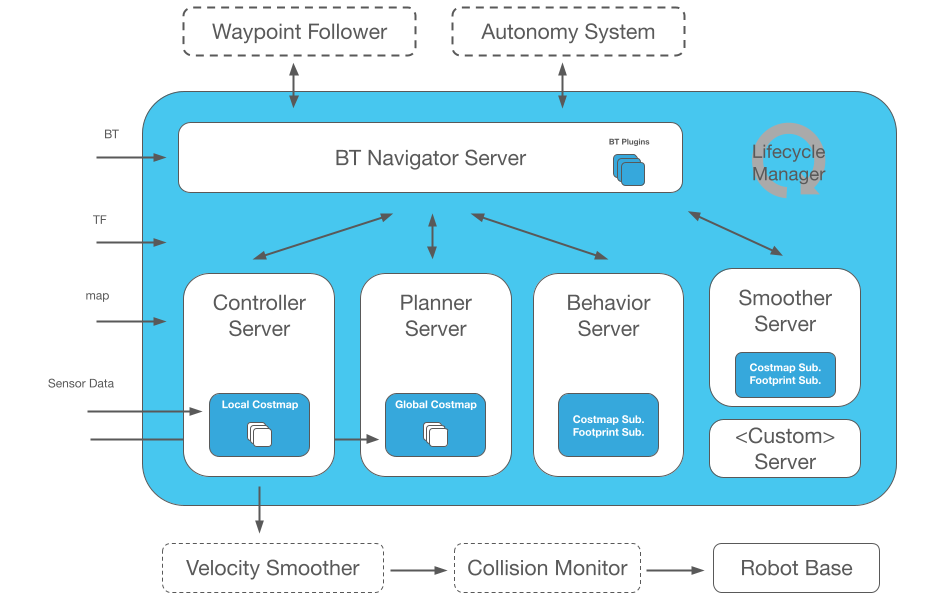
\includegraphics[width=0.9\paperwidth]{images/nav2_architecture}}
    \centering
    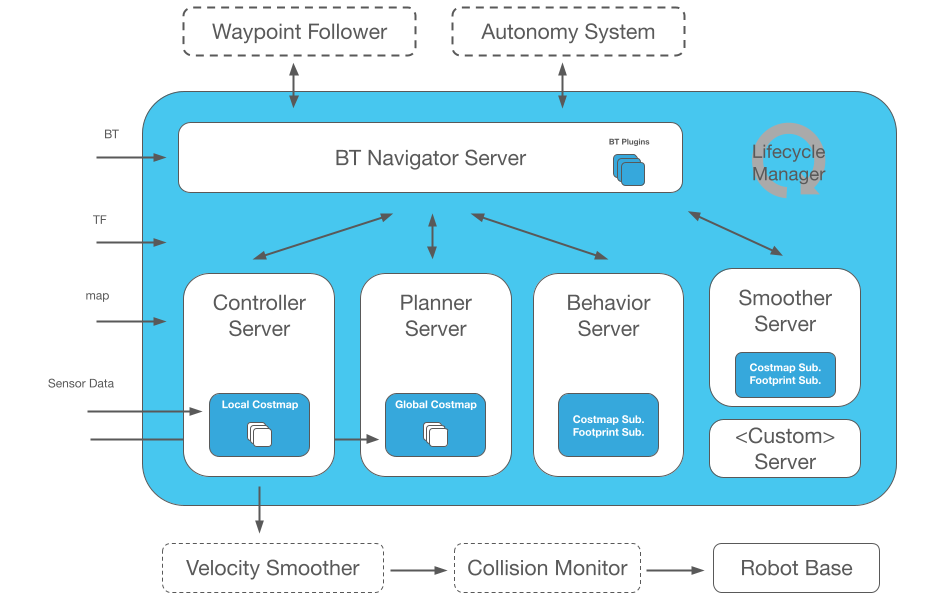
\includegraphics[width=0.8\textwidth]{images/nav2_architecture}
    \caption{Navigation architecture}
\end{figure}

\section{Docker}
  
\begin{wrapfigure}[3]{r}{0.15\textwidth}
    
\includegraphics[width=0.15\textwidth]{images/docker}
\end{wrapfigure}
  
Docker is a platform that let you separate your application using an isolated environment called container. It gives you also the possibility to run multiple containers at the same time. As it was originally designed, Docker was used in this project for the following reasons: % basta? (?)
  
\begin{itemize}
    \item \textbf{separate} this project workspace from all the other ones, to \textbf{avoid conflicts}
    \item keep the workspace \textbf{equal} for \textbf{every device} (real robot or simply a computer)
    \item permit development on any device \textbf{not running} necessarily \textbf{Ubuntu 20.04} (required from \acrshort{ros}2) as its OS
\end{itemize}  
  
Inside a Dockerfile, a file containing instructions on how to build an image\footnote{It is used as a starting point when launching a container} with your own configurations, were typed all the commands required to install the missing packages from the base image already containing basic \acrshort{ros}1 and \acrshort{ros}2 packages \cite{dockerimage}. The complete Dockerfile can be found in \autoref{cha:dockerfile}.
      % migliorare parte sotto (?)

\chapter{Working in a real environment}
\label{cha:realworld}

Talking about the real world, we need a real robot; the one used comes from the \acrfull{disi} of University of Trento.
A photo of the robot is shown in \autoref{fig:shelfino}. % (?)

\begin{figure}[h]
  \centering
  \includegraphics[width=0.6\textwidth]{images/nav2\_architecture}
  \caption{The, so called, \textit{shelfino} robot}
  \label{fig:shelfino}
\end{figure}

\section{Shelfino setup} 

\subsection{Adapting existing code}

The \textbf{hardware interface} was already developed by some research students in the last years, but they are no longer here. The original idea was to develop some ROS nodes that would connect to \textbf{encoders}, \textbf{motors drivers} and \textbf{lidar}, but specific information about brands or manufacturers of some of these components were not provided.

Another attempt was trying to rewrite the code in ROS2: it was not straightforward, and it did not work at the end, since the libraries used refers to a not well-known network infrastructure. Moreover, some feature has not been ported \textbf{equally} to \acrshort{ros}2, leading to some potential \textbf{differences} from the original code.

\subsection{\acrshort{ros}1 Bridge}

The final attempt involved the use of a \acrshort{ros}2 package called \textit{ros1\_bridge}. Since both \acrshort{ros}1 and \acrshort{ros}2 use their own \textbf{local network} to deliver messages, you can create a node that \textbf{listens to both networks} and when something is received from one side, it is sent to the other one: in this way it is possible to run the \textbf{existing code as it is} on a \acrshort{ros}1 node (with its dependencies), while making use of its topics and services on a \acrshort{ros}2 workspace at the same time.

But, in order to run both \acrshort{ros}1 and \acrshort{ros}2 nodes on the same machine (or Docker container), they need the same version of Ubuntu. \textbf{\acrshort{ros}2 Foxy} version is mandatory because of planning libraries, and runs only on \textbf{Ubuntu 20.04}, so also \acrshort{ros}1 has to use it; the original code, however, was written for the previous version (\acrshort{ros}1 Melodic, running only on Ubuntu 18.04), but luckily it runs without problems on the new one\footnote{The biggest change was introducing the support for Python 3}, \textbf{\acrshort{ros}1 Noetic} (for the same OS version).

To be more precise, it was used the \code{dynamic\_bridge} of this package, instead of \code{parametric\_bridge} and \code{static\_bridge} ones: with the first one you can choose what topics or services you want to bridge, but it has some bugs and does not work well, while the second one needs to be compiled every time there are some changes; the dynamic one, instead, adapts itself.

\subsection{Existing nodes explained}
\label{subsec:nodes}

In order to start the required nodes, a custom launch file was created. A launch file is a file containing information about \textbf{which nodes}, eventually with some \textbf{parameters}, should be \textbf{started} when the system is launched, instead of doing it one by one. Three nodes are inside this launch file:

\begin{itemize}
    \item \code{lidar\_position}
    \item \code{hw\_interface}
    \item \code{odom\_node}
\end{itemize}

\subsubsection{lidar\_position} % forse togliere e forse  mettere 0.43 (?)

\begin{lstlisting}[
  label={lst:lidarpos},
  language=xml,
  style=xmlStyle
  ]
  <node pkg="tf" type="static_transform_publisher" name="lidar_position"
    args="0 0 0.45 0 0 0 base_link lidar_link 100" />
\end{lstlisting}

This is a node (with a custom name) of the \code{tf} package of \acrshort{ros}1, \textit{a package that lets the user keep track of multiple coordinate frames over time [...] and lets the user transform points, vectors, etc. between any two coordinate frames at any desired point in time}. \cite{tf} The node executable is called \code{static\_transform\_publisher} and it is used to \textit{publish a static coordinate transform to tf using an x/y/z offset in meters and roll/pitch/yaw in radians [...]. The period, in milliseconds, specifies how often to send a transform}. \cite{tf} 
As \autoref{lst:lidarpos} shows, here it is used to describe the \textbf{transformation} between \code{base\_link}, the root frame (located on the ground under the robot, in the origin) and \code{lidar\_link} (0.45 meters above) every \code{100ms}. So when some points are returned by the laser scans, we also know the height, not otherwise specified, since it is a 2D scan.  

\subsubsection{hw\_interface}

It is a node designed to interface with the \textbf{underlying hardware}, thanks to the custom \code{hardwareglo\-balinterface} library previously developed by the researchers. It is a \textbf{helper class} using a \textbf{ZeroMQ framework} to deliver messages between the hardware (client) and the server running on the BeagleBone, that keeps track of the received data and make it accessible using the class methods.

Basically, using the just described interface, it reads the data coming from \textbf{encoders}, \textbf{lidar} and \textbf{tracking camera} and make it available as \acrshort{ros}2 topics (\code{/encoders, /scan, /t265}). It also subscribes to a \code{/cmd\_vel} topic from which reads the requested \textbf{linear} and \textbf{angular velocities} and dispatches them to the motors of the robot accordingly.

\subsubsection{odom\_node}

This node makes use of the information received from the \textbf{encoders topic} about the rotation of the wheels and \textbf{tracking camera topic}\footnote{A tracking camera is used in addition to wheels rotation to avoid odometry drift. If not using a tracking camera, when the robot is facing a wall and the wheels continue to rotate (and obviously the robot will not move), the odometry will tell the opposite, that it is still moving. When using it, if the robot is moving, certainly what the tracking camera perceives change, otherwise it will not, and it can be used to avoid what described above.} to calculate \textbf{odometry}, which represents an estimation of the \textbf{position} and the \textbf{rotation} of the robot from where it started. These new information are then published both as a message in a topic, and as a transformation between \code{odom\_frame} and \code{base\_link}, employed by the \textbf{navigation system} as described in \autoref{cha:navigation}.
      \chapter{Working in a simulated environment}
\label{cha:simworld}

\noindent\begin{wrapfigure}[16]{r}{0.3\textwidth}
    % \captionsetup{singlelinecheck = false, format= hang, justification=raggedright, labelsep=space}
    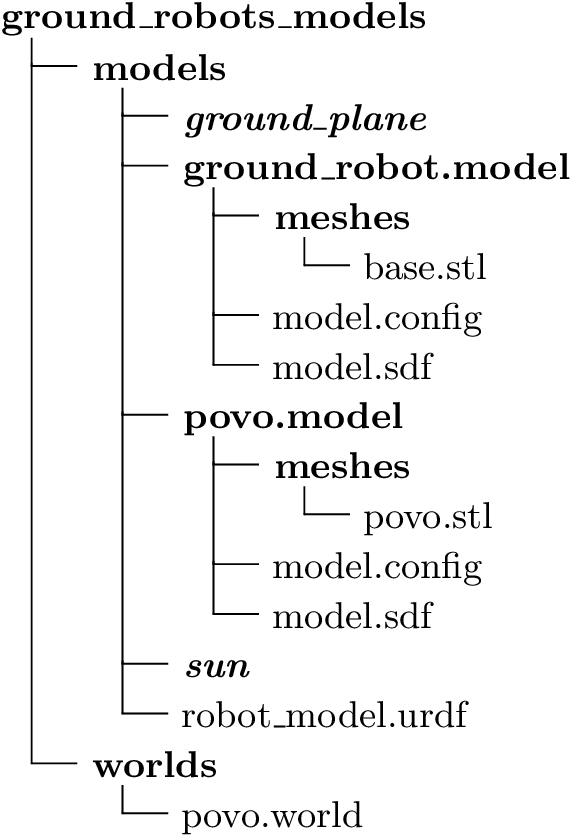
\includegraphics[width=0.3\textwidth]{images/models_folder}
    \caption{Models folder}
\end{wrapfigure}
The choice to develop a \textbf{simulation} is due to the fact that sometimes you may not physically be in university to use the real robot. The challenge here is to do a good job with \textbf{abstraction}, which means that the simulated robot and environment should be \textbf{as close as possible} to real ones. In other words, everything that used to work (i.e. navigation and planning) should now continue to work even if you are no longer in the real world; in theory you should not notice if you are in the real world or in a simulated one.

\section{Models}

To get a complete simulation, we need to create what is missing from reality, which environment and robot models.

\subsection{Environment}
\label{sub:map}

A mesh of the upper floors of Povo was provided by Professor \textit{Marco Roveri}\cite{roveri}. Unfortunately, compared to the navigation map generated by real data, it turns out that the mesh is \textbf{not very accurate}. Two workarounds are possible: create a \textbf{new navigation map} for simulation purposes or \textbf{adapt the mesh} to the real environment with some modifications; it turns out, as described in \autoref{sub:waypoints}, that already only by scaling up one side of the mesh, you get a better result. 

A model is then created using \acrfull{sdf} and later inserted inside a \code{world} file\footnote{A collection of the models you want to display in the Gazebo scene, always written in \acrshort{sdf}}.

\begin{figure}[h]
    \centering
    \includegraphics[width=0.8\textwidth]{images/3d\_povo\_model}
    \caption{Povo model for simulation. Colors were used for a better visualization.}
\end{figure}

\subsection{Robot}
\label{sub:robot}

Part of the setup is inspired to \textit{Automatic Addison} tutorials\cite{tutorials}.

The robot mesh was created starting from the \textit{shelfino} shape (see \autoref{fig:shelfino}), trying to keep it \textbf{as similar as possible}, and each piece (robot base, lidar, wheels and caster wheel) was exported singularly. For performance reasons in Gazebo, the only mesh actually used is the robot base, because of its special structure to \textbf{avoid contact} with the wheels \textbf{partially inside}. The other ones are replaced by \acrshort{sdf} or \acrfull{urdf} built-in geometric shapes (i.e. cylinders).
Both \acrshort{sdf} and \acrshort{urdf} files have been used: the first one for Gazebo and the second one for a node called \code{robot\_state\_publisher} that helps to visualize the robot in \acrshort{rviz}.

\begin{figure}[h]
    \centering
    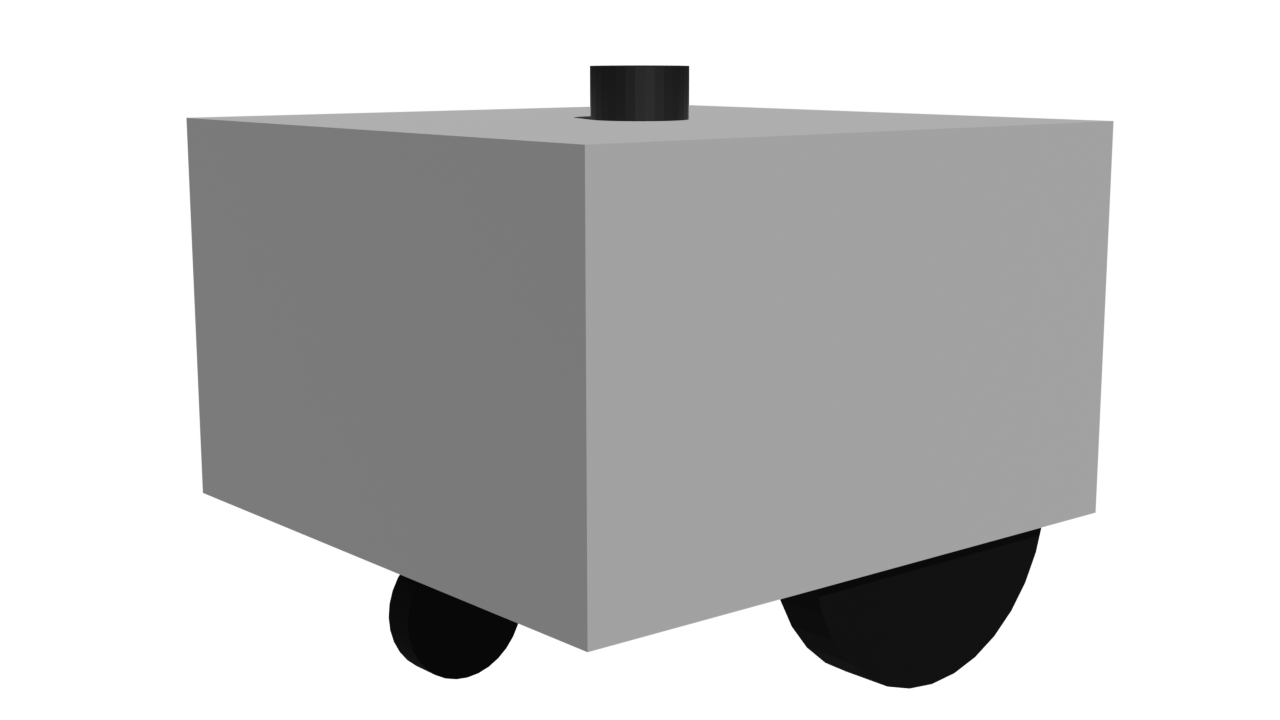
\includegraphics[width=0.7\textwidth]{images/shelfino_3d.png}
    \caption{Shelfino model for simulation.}
\end{figure}

\section{Gazebo plugins}

After placing the models in Gazebo, we need a way for our robot \textbf{interact} to interact with the environment. You can no longer utilize the nodes in \autoref{subsec:nodes} because they make use of a real hardware, but thankfully Gazebo provides some \textbf{plugins} that can be added to the \acrshort{sdf} model as a normal tag. We always need a way to set the \textbf{linear and angular velocities} to make the robot moves as desired, a way to \textbf{calculate odometry} and a lidar to \textbf{detect obstacles}. Once done, the robot can be used as if it were a real robot.

Sadly, there are no plugins available for tracking cameras, so we content ourselves with only wheels rotation information to calculate odometry. 

\subsection{Differential drive plugin}

Once added, some configurations needs to be made:
\begin{itemize}
    \item set \textbf{update rate} (Hz)
    \item specify \textbf{name} of wheel joints (control)
    \item set wheels \textbf{separation} and \textbf{diameter} (kinematics)
    \item set max \textbf{torque} and \textbf{acceleration} (limits)
    \item specify topic names from where \textbf{receiving desired velocity} and \textbf{publish odometry data}
    \item whether to \textbf{publish frame transformations} and their names (used by \acrshort{rviz})
\end{itemize}
Now, the robot can move.

\subsection{Ray sensor plugin}

To allow the robot to able to detect obstacles, a lidar is required. To do so, you can simpy use the Gazebo \textbf{sensor} \code{ray} tag, setting \textbf{scan}, \textbf{range} and \textbf{noise} information, but even a plugin is required to make it work. The only necessary configurations are:
\begin{itemize}
    \item which \acrshort{ros} message type to use as \textbf{output} (\code{sensor\_msgs/LaserScan})
    \item frame name to which the lidar is \textbf{attacched} (described elsewhere else in the model)
\end{itemize}
      \chapter{Navigation}

\def\code#1{\texttt{#1}}

% Everything required to navigate through the environment is provided by \code{g\_robot} package. The complete structure is shown in the following figure.

% \begin{wrapfigure}{l}{0.3\textwidth}
%   \captionsetup{singlelinecheck = false, format= hang, justification=raggedright, font=footnotesize, labelsep=space}
%   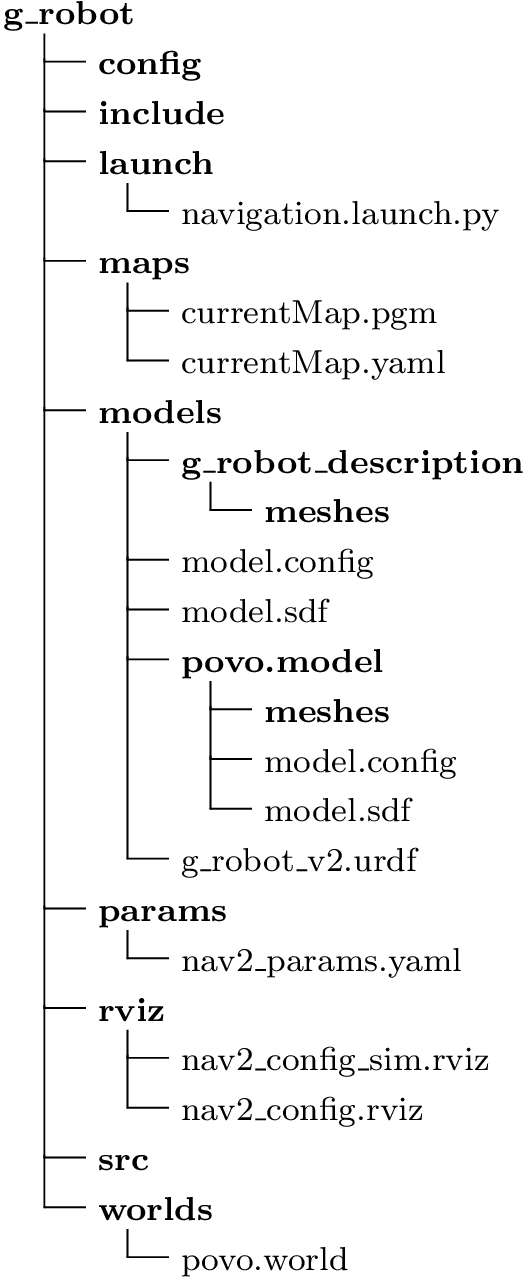
\includegraphics[width=0.3\textwidth]{g-robot}
%   \caption{Folder structure of the g\_robot package}
% \end{wrapfigure}

As described in \autoref{cha:techstack}, for the navigation part it was used the \Acrshort{nav2} package. 
      \chapter{Planning integration} % add folder structure
\label{cha:planningbridge}

This chapter aims to \textbf{integrate} the planning part developed by \textit{Filippo Rossi}\footnote{His entire project is described in \autoref{sub:planning}} \cite{fr}. What already discussed in the previous chapters leads to a \textbf{working} version of the robot (it is able to move around), but does not have any practical use, because you need to set \textbf{where} you want the robot to go \textbf{every time}. This is the goal of this chapter: add some \textbf{missions control} (?), to give the robot some tasks it has to complete, without the needing of any \textbf{low-level human interaction}.

\section{Modifications from original planning}

When the planning was developed, Filippo could not receive any feedback, since we were facing some other challenges (i.e. make robots move autonomously). So, in response, the planning is more like a \textbf{generic workspace} to which we can add some \textbf{modifications} to meet our specific needs; then we can attach the \textbf{adapted workspace} to what was already developed, since \acrshort{ros} is \textbf{modular}.

% aggiungere entrance tag per entrata porta, dato che non è ben definita

\subsection{Change JSON structure}
\label{sub:json}

Thanks to Filippo's \textbf{waypoints extractor} and \code{cvat} \textbf{annotation software}, all the coordinate information can be found in a \textbf{JSON file}: when the robot is told to move in a certain room, only step to take is \textbf{searching} its name in the file and reading its \textbf{coordinates}.

But, because this JSON file was written as a \textbf{list of dictionaries}, it would be required to iterate \textbf{over every element} and search for the one with the \textbf{requested name}, and when they match, it is possible to get the coordinates. Instead, for an easier use, a dictionary is created with the name of the room as \textbf{key} and the coordinates of its center and its boundaries as \textbf{value}. Also, coordinates on Z axis are removed since they are shared among all rooms. A comparison is shown in \autoref{lst:origjson} and \autoref{lst:modjson}. This operation has been performed with the \code{Python} script shown in \autoref{lst:script}.

\noindent\begin{minipage}{0.425\textwidth}
\noindent\begin{lstlisting}[
    language=json,
    style=jsonStile,
    caption={Original JSON structure},
    label={lst:origjson}]
[
    {
        "label": "povo_1_258",
        "center": [
            -11.749180327868853,
            -35.01639344262295,
            1.5
        ],
        "max": [
            -8.0,
            -30.5,
            1.5
        ],
        "min": [
            -15.5,
            -40.0,
            1.5
        ]
    },
    ...
]
\end{lstlisting}
\end{minipage}
\noindent\begin{minipage}{0.15\textwidth}
    \centering
    \noindent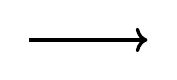
\begin{tikzpicture}
        \draw[->, very thick] (0,0) -- (1.5,0);
    \end{tikzpicture}
\end{minipage}
\noindent\begin{minipage}{0.425\textwidth}
\noindent\begin{lstlisting}[
    language=json,
    style=jsonStile,
    caption={Modified JSON structure},
    label={lst:modjson}]

{
    "povo_1_258": {
        "center": [
            -11.749180327868853,
            -35.01639344262295

        ],
        "max": [
            -8.0,
            -30.5

        ],
        "min": [
            -15.5,
            -40.0

        ]
    },
    ...
}
\end{lstlisting}
\end{minipage}


\subsection{Correct waypoint coordinates}
\label{sub:waypoints}

In order to generate those waypoints inside the JSON file, Filippo used the same mesh described in \autoref{sub:map}, and, as already discussed, it does not match perfectly the real environment. Furthermore, the navigation map is rotated with respect to the mesh.

So, using \textit{Blender} \cite{blender}, after loading both mesh and map, some \textbf{modifications} that lead to a \textbf{better result} have been found: \textbf{turn} the mesh around the Z axis, \textbf{scale} it up the long side (Y axis), and \textbf{translate} it along both sides. Luckily, when applying these transformations on the entire mesh, it is like doing it on those JSON waypoints, without needing to repeat the annotation process from the beginning. These \textit{transformations} have been performed with the Python script showed in \autoref{lst:script}

\applymulticoltrue

\noindent\begin{lstlisting}[
    language=Python,
    style=PythonStile,
    caption={Python example script used to transform waypoint coordinates},
    label={lst:script}]
...
import numpy as np

translation = np.array([6.8210, 8.7180, 0])
rot_z = 135 * np.pi / 180
scale_y = 1.0925
...
rot_matrix = np.array(
    [[np.cos(rot_z), -np.sin(rot_z), 0],
     [np.sin(rot_z), np.cos(rot_z), 0],
     [0, 0, 1]])

scale_matrix = np.array([[1, 0, 0], 
                         [0, scale_y, 0],
                         [0, 0, 1]])

roto_scaling = np.dot(rot_matrix, scale_matrix)

# iterate over each element of the original list (original_data) and save all keys and values in a new dict (dict_data)
for obj in original_data:
    dict_data[obj["label"]] = {
        k: (-translation-np.dot(-roto_scaling, np.array(v)))[0:2].tolist()
        for k, v in obj.items()
        if k != "label"
    }
...
\end{lstlisting}

\applymulticolfalse

Rotation and scale matrices are calculated and \textbf{fused} together. Then, as described in \autoref{sub:json}, the JSON structure is \textbf{changed} with dictionaries and each value of its corresponding key is transformed by applying the rotation-scale matrix and the translation vector. At the end, with \code{[0:2]}, only x and y coordinates are kept.

\subsection{Remove stub nodes from execution}

Currently, the only actions supported are \code{ugv\_move} and \code{ugv\_transporting\_uav\_move}: although the name is different, they share the \textbf{same code} (they have been separated for planning reasons). For testing purposes, in the original planning some nodes were added to simulate \acrshort{ugvs} and \acrshort{uavs}: they were started at the beginning of the execution, but now these two have their real implementation, so the \textbf{stub ones} have been removed from the launch.

\section{Task executors}

Four nodes have been created and are started together to let the robot moves autonomously: 
\begin{itemize}
    \item \arguments{navigation client}{service and action client that sets the navigation goal when coordinates are received}
    \item \arguments{pose server}{service server responsible for returning the current pose of the robot when requested}
    \item \textbf{two planning clients} (\code{ugv\_move}\footnote{\label{fn:node}Node name is equal to action name} and \code{ugv\_transporting\_uav\_move}\footnoteref{fn:node}): \textit{action executor clients listening for next action to complete}
\end{itemize}

The entire workflow is shown in \autoref{fig:bridge}. A more detailed one can be found in Attachment \ref{cha:deepening}.

\begin{figure}[h]
    \centering
    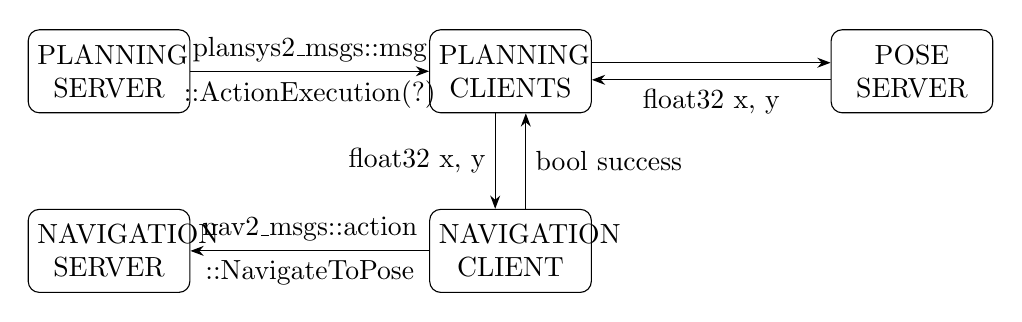
\begin{tikzpicture}
        \node [block] (plan-server) {PLANNING SERVER};
        \node [block, below=of plan-server] (nav-server) {NAVIGATION SERVER};
        \node [block, right=of plan-server] (plan-clients) {PLANNING CLIENTS};
        \node [block, right=of nav-server] (nav-client) {NAVIGATION CLIENT};
        \node [block, right=of plan-clients] (pose-server) {POSE SERVER};

        \draw [arrow] (plan-server) -- node [above] {plansys2\_msgs::msg} node [below] {::ActionExecution(?)} (plan-clients);
        \draw [arrow] (nav-client) -- node [above] {nav2\_msgs::action} node [below] {::NavigateToPose} (nav-server);
        \draw [arrow] (plan-clients.250) -- node [left] {float32 x, y} (nav-client.110);
        \draw [arrow] (nav-client.70) -- node [right] {bool success} (plan-clients.290);
        \draw [arrow] (plan-clients.6) -- (pose-server.174);
        \draw [arrow] (pose-server.186) -- node [below] {float32 x, y} (plan-clients.354);
    \end{tikzpicture}
    \caption[Nodes interaction]{
        On the left, the already existing servers, in the center, the custom clients written, and on the right, the custom server written. On the arrows, the messages exchanged.
    }
    \label{fig:bridge}
\end{figure}

\subsection{Navigation client}

This node is both a \textbf{service server} and an \textbf{action client}: the first one is used to receive the coordinates from the planning clients, and then, using the second one, it connects to the navigation action server and sets the just received goal. It is called only \textbf{once}, when a new task is created.

\subsection{Pose server}
\label{sub:pose}

When it receives a request, it returns the \textbf{current position} of the robot, which is \code{base\_link} position in the \code{map} frame. In order to achieve it, some other calculations need to be done: we are interested in \code{base\_link} frame, but the only transformation referring (to it) is the \code{odom} one, not the same used for waypoint coordinates. There is the need to express it from the \code{map} frame perspective, and luckily such a transformation (\code{map} $\rightarrow$ \code{odom}) is available thanks to \acrshort{amcl} node. 
Thanks to \code{tf\_echo} node \cite{tfexample} used as a template\footnote{If you follow the documentation, the process to get the transformation between two frames not directly connected, it will not work. The only node doing this and also working is \code{tf\_echo}.}, it was possible to obtain the correct transformation, \textbf{fusing} the required two.

\subsection{Planning clients}

It is an \textbf{action client} (called \code{ActionExecutorClient}), coming from \code{plansys2\_executor} (cite (?)) package, of \code{plansys2\_msgs::action::ExecuteAction} action: it means that it connect to its server (called \code{ActionExecutor}) waiting for a \textbf{new goal} to reach. When it received a new goal is responsible for completing it, and at the same time he has to return \textbf{continuous feedback
} with the current percentage of completion, until the goal is \textbf{reached} (100\% completion).

When a new task has been created and started, the action server would call the \code{do\_work()} method of the designed client, to let it know a new job needs to be completed.
Inside this method the client transforms the \textbf{room name} (passed as goal) in \textbf{coordinates} and, if the goal was not already set, it passes it to the navigation client, making use of a custom service. After that, it asks \textbf{its current position} to the pose server (with another service) and uses it to set both the \textbf{initial and current position} (because the robot is not moving yet, the current position is the same as the initial one); using them, it returns a \textbf{percentage of completion} (0\%) to the planning server.

The \code{do\_work()} method, then, is called \textbf{continuously} until the task is completed to give some feedback: now the initial position is already set (and as a result also the goal), so it continues to ask only for its current position, to calculate the \textbf{euclidean distance} from the initial position and then, it returns a new percentage of completion.

\begin{wrapfigure}{r}{0.25\textwidth}
    \begin{equation*}
        1-\dfrac{current\_distance}{initial\_distance}
    \end{equation*}
    \caption{Percentage of completion}
    \label{eq:percentage}
\end{wrapfigure} 

Because the path used to reach the destination might not be \textbf{a straight line} and the distance employed is the euclidean one, it could happen the current distance is \textbf{greater} than the initial one: 
in this case, they are swapped to keep 0\% as the \textbf{lower bound} of completion, otherwise it would become negative. Choosing the maximum between percentage of completion and zero would lead to \textbf{loss of information}, and it is the reason why it has not been used. This can be clearly seen in \autoref{eq:percentage}.
      \chapter{Results and Future works}
\label{cha:futureworks} %(?)

\section{Conclusion}

At the end, the robot, whether real o simulated, is able to \textbf{navigate} the environment, detect \textbf{obstacles} and take actions to \textbf{avoid} them. Moreover, he can also move \textbf{autonomously} from one room to another, without having to control the robot manually (setting yourself the destination). When also the drone project have been completed and tested, it will be possible to \textbf{join} everything together and have a \textbf{complete system} as designated originally.

\section{Further improvements}

Here it is a possible list of missing or incomplete features that can be implemented in the future:

\begin{itemize}

\item Currently, of three \textit{shelfino} robots, two are working, and only one is \textbf{accessible} through the network, necessary to set it up for the current project: although it should have been a multi-robot system, it has only been tested with one, for obvious reasons. Once this issue is resolved, a multi-robot test could be performed.

\item Because of \textbf{asynchronous} development of each project, on the planning part was assumed that only \acrshort{uavs} are capable of \textbf{taking photos}, even if it could be done also with \acrshort{ugvs}: the implementation would be quite straightforward. Right now, \acrshort{ugvs} are only moving around, without a surveillance task, except for carrying \acrshort{uavs}. (?) 

\item From the specific actions designed for \acrshort{ugvs}, only \code{movement} and \code{move\_with\_uav} ones were implemented, as opposed to \code{battery\_managment} and \code{charge} operations, because there is \textbf{no way} to interface with batteries and auto-charging them is not possible since a \textbf{missing infrastructure} is needed; in other words, such actions, are possible only manually (with voltmeter and cables).

\item A fancy feature that could be supported, as soon as it has been fully implemented on the planning system, is \textbf{live positioning}: in this way you could have a \textbf{real-time position feedback} also in the web interface; the only change consists on returning also the position of the robot\footnote{gotten from the pose server, described in \autoref{sub:pose}} alongside the current task completion percentage.

% \item Talking about the navigation part, the obstacle avoidance could be enhanced, especially in the case of dynamic obstacles, because the robot sometimes takes some time to figure out what is going on and could end up colliding with them. A possible workaround could be increasing the minimum distance that should be kept between the robot and the unexpected obstacle, with some recovery action, like going back and replanning the path. A problem could also be the \code{ros1\_bridge} that adds some delay when exchanging messages between \acrshort{ros}1 and \acrshort{ros}2, ending up receiving lidar data not instantaneously. (?)

\item Improve the map, creating a custom one for simulation and keeping the current (or creating a more complete) one for the real world. If a better mesh is available, \acrshort{slam} and waypoint generation in simulation and real world would be the same, and then you do not have to \textbf{switch} from one to another every time.

% \item Add docker compose (?)

\end{itemize}
      
    \endgroup

    % bibliografia in formato bibtex
    %
    % aggiunta del capitolo nell'indice
    \addcontentsline{toc}{chapter}{Bibliografia}
    % stile con ordinamento alfabetico in funzione degli autori
    \bibliographystyle{plain}
    \bibliography{biblio}

    \titleformat{\chapter}
        {\normalfont\Huge\bfseries}{Attachment \thechapter}{1em}{}
    % sezione Allegati - opzionale
    \appendix
    \chapter{Planning Bridge deepening}
\label{cha:deepening}

\newsavebox\poseserver

\noindent\begin{lrbox}{\poseserver}
  \noindent\begin{lstlisting}[language=C, style=CStyleTextWidth]
while (rclcpp::ok() && !listener_.buffer_.canTransform("map", "base_link", tf2::TimePoint())) rate.sleep();

geometry_msgs::msg::TransformStamped transform_ = listener_.buffer_.lookupTransform("map",  "base_link", tf2::TimePoint());

response->x = transform_.transform.translation.x;
response->y = transform_.transform.translation.y;
  \end{lstlisting}
\end{lrbox}

\newsavebox\navigationclient

\noindent\begin{lrbox}{\navigationclient}
  \noindent\begin{lstlisting}[language=C, style=CStyleNoFrame]
goal_->pose.position.x = request->x;
goal_->pose.position.y = request->y;
goal_->pose.position.z = 0;
goal_->pose.orientation.x = 0.0;
goal_->pose.orientation.y = 0.0;
goal_->pose.orientation.z = 0.0;
goal_->pose.orientation.w = 1.0;
goal_->header.frame_id = "map";
goal_->header.stamp = now();
send_goal();
response->success = true;
  \end{lstlisting}
\end{lrbox}

\noindent\begin{figure}[h]
  \centering
    \noindent\begin{tikzpicture}
      \node [poseserver] (pose-server) {\usebox\poseserver};
      \node[fill=white] at (pose-server.south) {POSE SERVER};
      
      \node [inception, above left=5.7cm and -4.625cm of pose-server] (do-work) {DO WORK};
      \node [inception, above left=3.8cm and -4.625cm of pose-server] (get-pose) {GET POSE};
      \node [inception, above left=1.9cm and -4.625cm of pose-server] (continue-work) {CONTINUE WORK};
      \node[inception, inner xsep=1em, inner ysep=1em, fit=(do-work) (continue-work), above left=1.5cm and -5cm of pose-server] (plan-clients) {};
      % \node [poseserver, above=1cm of pose-server, fit=(do-work) (continue-work)] (plan-clients) {PLANNING CLIENTS};  
      \node[fill=white] at (plan-clients.south) {PLANNING CLIENTS};

      \node [navigationclient, right=5cm of plan-clients] (nav-client) {\usebox\navigationclient};
      \node[fill=white] at (nav-client.south) {NAVIGATION CLIENT};

      \node [block, above=3cm of plan-clients] (plan-server) {PLANNING SERVER};
      \node [block, right=7.9cm of plan-server] (nav-server) {NAVIGATION SERVER};

      \draw [arrow] (plan-server) -- node [left] {plansys2\_msgs} node [right] {::msg::ActionExecution} (plan-clients);
      \draw [arrow] (nav-client) -- node [left] {nav2\_msgs::action} node [right] {::NavigateToPose} (nav-server);
      \draw [arrow] (do-work.7) -- node [above] {float32 x, y} (nav-client.148);
      \draw [arrow] (nav-client.154) -- node [below] {bool success} (do-work.353);
      \draw [arrow] (get-pose.353) -| (pose-server.95);
      \draw [arrow] (pose-server.85) |- node [above left] {float32 x, y} (get-pose.7);

      \draw [arrow] (do-work) -- (get-pose);
      \draw [arrow] (get-pose) -- (continue-work);

  \end{tikzpicture}
  \caption[Nodes interaction deepening]{\textbf{DO WORK}, \textbf{GET POSE} and \textbf{CONTINUE WORK} functions are shown in the next page.}
\end{figure}

\newpage

\subsection{DO WORK function}

\noindent\begin{lstlisting}[language=C, style=CStyle, caption={Starts navigation with the given goal coordinates}]
if(!is_initial_distance_set_){
  room_goal_ = current_arguments_[GOAL_INDEX];
  goal_position_ = labels_.at(room_goal_).at("center").get<std::vector<double>>();
  
  auto request = std::make_shared<planning_bridge_msgs::srv::StartNavigation::Request>();
  request->x = goal_position_[0];
  request->y = goal_position_[1];
  
  start_navigation_client_->async_send_request(request,
  [this](rclcpp::Client<planning_bridge_msgs::srv::StartNavigation>::SharedFuture future){
    auto result = future.get();
    if(result->success) {
      RCLCPP_INFO(get_logger(), "Navigation started");
      get_pose();
    } else {
      RCLCPP_ERROR(get_logger(), "Navigation failed");
    }
  });
  
} else {
  get_pose();
}
\end{lstlisting}

\subsection{GET POSE function}

\noindent\begin{lstlisting}[language=C, style=CStyle, caption={Asks pose and sets initial and current poses}]
current_pose_client_ptr_->async_send_request(
  std::make_unique<planning_bridge_msgs::srv::CurrentPose::Request>(),
  [this](rclcpp::Client<planning_bridge_msgs::srv::CurrentPose>::SharedFuture future) {
    auto result = future.get();
    if(!is_initial_distance_set_){
      initial_distance_ = std::sqrt(std::pow(result->x - goal_position_[0], 2) +
      std::pow(result->y - goal_position_[1], 2));
      is_initial_distance_set_ = true;
      current_distance_ = initial_distance_;
    } else {
      current_distance_ = std::sqrt(std::pow(result->x - goal_position_[0], 2) +
      std::pow(result->y - goal_position_[1], 2));
      if(current_distance_ > initial_distance_){
        float temp = current_distance_;
        current_distance_ = initial_distance_;
        initial_distance_ = temp;
      }
    }
    continue_work();
    });
\end{lstlisting}

\newpage

\subsection{CONTINUE WORK function}

\noindent\begin{lstlisting}[language=C, style=CStyle, caption={Sends feedback until the goal is reached}]
progress_ = 1.0 - (current_distance_ /
initial_distance_);

if (progress_ < 0.95) {
  send_feedback(progress_, "Move running");
} else {
  finish(true, 1.0, "Move completed");

  progress_ = 0.0;
  is_initial_distance_set_ = false;
  std::cout << std::endl;
}

std::cout << "\r\e[K" << std::flush;
std::cout << "Moving ... [" << std::min(100.0, progress_ * 100.0) << "%]" << std::flush;
  \end{lstlisting}

\chapter{How to}

As described in \autoref{cha:techstack}, \code{docker compose} has been used in order to easily \textbf{deploy} the system. However, \textbf{several configurations} are available (e.g. run everything on the robot, run only robot nodes on the robot, run \acrshort{slam}, run simulation), and you should edit the \code{docker-compose.yaml} file each time to meet your needs, or have multiple files containing different configurations. To simplify it, some Python scripts have been created:

\begin{itemize}
  \item \code{start.py}
  \item \code{attach.py}
  \item \code{stop.py}
\end{itemize}

\subsection{start.py}

\begin{lstlisting}[language=bash, style=bashStyle, caption={Generates a \code{docker-compose.yaml} file from a template and runs it}]
usage: start.py [-h] [-r] [-g] [-n] [-s] [-m] [-p] [-d]

start desired nodes containers

optional arguments:
  -h, --help         show this help message and exit
  -r, --robot        start robot nodes
  -g, --gazebo       start simulation nodes
  -n, --navigation  start navigation nodes
  -s, --slam         start slam nodes
  -m, --map          save slam map
  -p, --planning     start planning nodes
  -d, --detached     run containers in detached mode
\end{lstlisting}

\noindent You can decide \textbf{which nodes} you want to run by passing the corresponding arguments\footnote{Some of them may be mutually exclusive}. Note that each time, before running the actual nodes, the workspace will be \textbf{recompiled}, to include any latest changes.

\subsection{attach.py}

\begin{lstlisting}[language=bash, style=bashStyle]
usage: attach.py [-h] [-r | -b | -g | -n | -s | -m | -p | -u | -w]

attach to a desired container

optional arguments:
  -h, --help         show this help message and exit
  -r, --robot        attach to robot container
  -b, --bridge       attach to ROS1-ROS2 bridge node
  -g, --gazebo       attach to simulation container
  -n, --navigation  attach to navigation container
  -s, --slam         attach to slam container
  -m, --map          attach to map container
  -p, --planning     attach to planning container
  -u, --ugv          attach to UGV actions container
  -w, --webserver    attach to webserver container  
\end{lstlisting} 

\noindent It is possible to attach to only one container at a time, since each argument is \textbf{mutually exclusive}. This is useful to \textbf{debug} the system, or to \textbf{run commands} inside the container.

\subsection{stop.py}

\begin{lstlisting}[language=bash, style=bashStyle]
usage: remove.py [-h]

remove running or stopped containers

optional arguments:
  -h, --help  show this help message and exit
\end{lstlisting}
    
    \clearpage
    \addcontentsline{toc}{chapter}{Acronyms}
    \printnoidxglossaries

% \end{slashbreak}
\end{document}